\documentclass[10pt]{beamer}
\usepackage{graphicx}
\usepackage{hyperref}
\usepackage{xcolor}
\usepackage{tikz}
\usepackage{amsmath}
\usetikzlibrary{shapes.geometric, arrows, positioning, fit, calc, shadows, decorations.pathmorphing, patterns, chains, scopes}

% --- A clean, minimalist theme that maximizes content space ---
\usetheme{Boadilla}
\usecolortheme{default}

% --- TikZ Style Definitions for Diagrams ---
\tikzstyle{block} = [rectangle, draw, fill=blue!20, text width=6em, text centered, rounded corners, minimum height=3em]
\tikzstyle{wideblock} = [rectangle, draw, fill=blue!20, text width=12em, text centered, rounded corners, minimum height=3em]
\tikzstyle{line} = [draw, -latex']
\tikzstyle{highlight} = [rectangle, rounded corners, fill=red!20, draw=red, thick, drop shadow]
\tikzstyle{note} = [text width=8em, text centered, font=\small]
\tikzstyle{arrow} = [thick,->,>=stealth]
\tikzstyle{smallblock} = [rectangle, draw, fill=gray!20, minimum height=1.5em, text width=7em, font=\tiny, text centered]

% --- Remove distracting elements to maximize content area ---
\setbeamertemplate{navigation symbols}{}
\setbeamertemplate{footline}[frame number] % Keep only a simple frame number
\setbeamertemplate{headline}{}

% --- Title Information ---
\title[LLM Agent Debugging]{A Comprehensive Guide to LLM Agent Debugging}
\author{Gemini Agent}
\institute{An Exhaustive Walkthrough of AgentDebug (Zhu et al., 2025)}
\date{\today}


\begin{document}

% --- TITLE SLIDE ---
\begin{frame}
  \titlepage
\end{frame}

% --- AGENDA ---
\begin{frame}
  \frametitle{Presentation Agenda}
  \begin{enumerate}
    \item Understanding the Agent's World: Trajectories \& Failures
    \item A Deep Dive into the \texttt{AgentErrorTaxonomy}
    \begin{itemize}
        \item Methodology
        \item Complete breakdown of all 5 modules and their error types
    \end{itemize}
    \item The \texttt{AgentDebug} Framework: A Step-by-Step Guide
    \item Experimental Validation: Does it Work?
    \item Illustrative Cases from Multi-Agent Systems (\texttt{MAST})
    \item Conclusion \& Key Takeaways
  \end{enumerate}
\end{frame}

% --- PART 1: CORE CONCEPTS ---
\part{Core Concepts: Trajectories \& Failures}

\begin{frame}
  \frametitle{Visualizing an Agent's Trajectory}
  A \textbf{trajectory} is the complete log of an agent's attempt to solve a task. It's a sequence of steps, where each step contains the agent's entire reasoning process.
  
  \begin{center}
  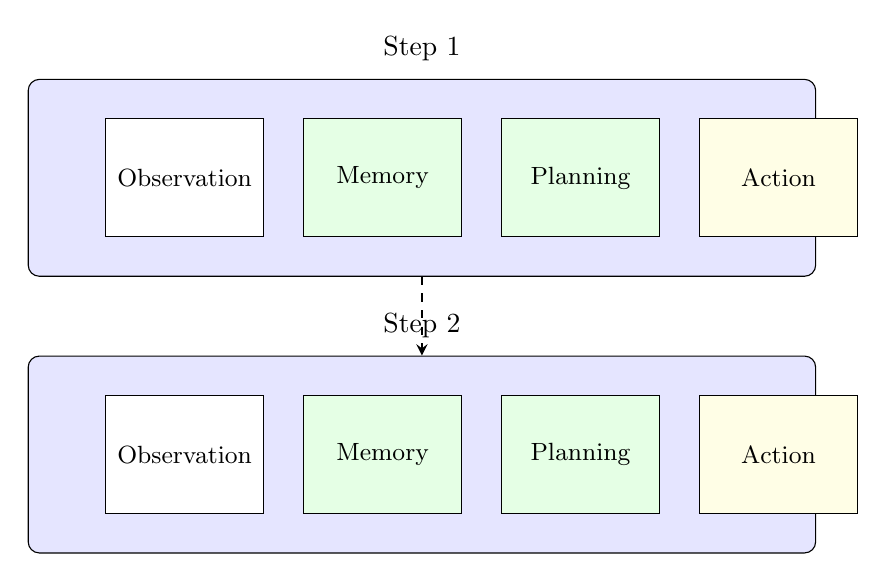
\begin{tikzpicture}[
    stepnode/.style={rectangle, draw, rounded corners, fill=blue!10, minimum width=10cm, minimum height=2.5cm},
    module/.style={rectangle, draw, fill=white, minimum width=2cm, minimum height=1.5cm, text centered, font=\small},
    node distance=0.2cm and 0.5cm
  ]
    % Step 1
    \node[stepnode] (step1) {};
    \node[module, left=of step1, xshift=3.5cm] (obs1) {Observation};
    \node[module, fill=green!10, right=of obs1] (mem1) {Memory};
    \node[module, fill=green!10, right=of mem1] (plan1) {Planning};
    \node[module, fill=yellow!10, right=of plan1] (act1) {Action};
    \node[above=0.1cm of step1] {Step 1};

    % Step 2
    \node[stepnode, below=1cm of step1] (step2) {};
    \node[module, left=of step2, xshift=3.5cm] (obs2) {Observation};
    \node[module, fill=green!10, right=of obs2] (mem2) {Memory};
    \node[module, fill=green!10, right=of mem2] (plan2) {Planning};
    \node[module, fill=yellow!10, right=of plan2] (act2) {Action};
    \node[above=0.1cm of step2] {Step 2};
    
    \draw[arrow, thick, dashed] (step1) -- (step2);
  \end{tikzpicture}
  \end{center}
\end{frame}

\begin{frame}
  \frametitle{How and Where Failures Appear in a Trajectory}
  A single flaw in one module can corrupt the entire rest of the step, and cascade into future steps.
  
  \begin{center}
  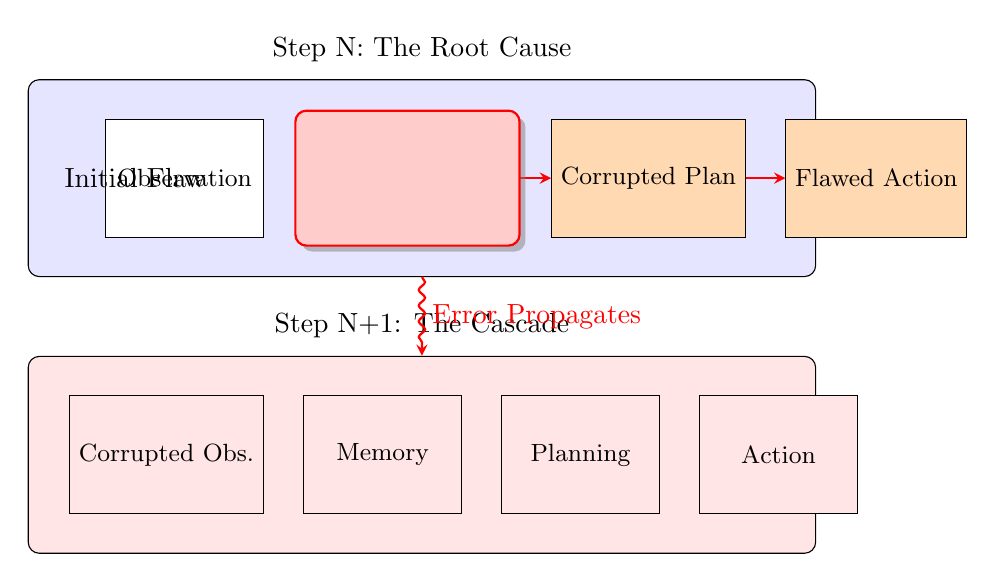
\begin{tikzpicture}[
    stepnode/.style={rectangle, draw, rounded corners, fill=blue!10, minimum width=10cm, minimum height=2.5cm},
    module/.style={rectangle, draw, fill=white, minimum width=2cm, minimum height=1.5cm, text centered, font=\small},
    node distance=0.2cm and 0.5cm
  ]
    % Step N
    \node[stepnode] (stepN) {};
    \node[module, left=of stepN, xshift=3.5cm] (obsN) {Observation};
    \node[module, fill=red!30, right=of obsN] (memN) {\textbf{Memory Error}};
    \node[module, fill=orange!30, right=of memN] (planN) {Corrupted Plan};
    \node[module, fill=orange!30, right=of planN] (actN) {Flawed Action};
    \node[above=0.1cm of stepN] {Step N: The Root Cause};
    
    % Arrows for Step N
    \draw[arrow, red, thick] (memN) -- (planN);
    \draw[arrow, red, thick] (planN) -- (actN);

    % Step N+1
    \node[stepnode, fill=red!10, below=1cm of stepN] (stepN1) {};
    \node[module, fill=red!10, left=of stepN1, xshift=3.5cm] (obsN1) {Corrupted Obs.};
    \node[module, fill=red!10, right=of obsN1] (memN1) {Memory};
    \node[module, fill=red!10, right=of memN1] (planN1) {Planning};
    \node[module, fill=red!10, right=of planN1] (actN1) {Action};
    \node[above=0.1cm of stepN1] {Step N+1: The Cascade};
    
    \draw[arrow, thick, red, decorate, decoration={snake,amplitude=.4mm,segment length=2mm,post length=1mm}] (stepN) -- node[right, pos=0.5] {Error Propagates} (stepN1);
    
    \node[highlight, fit=(memN), inner sep=0.1cm, label={[xshift=-1cm]left:Initial Flaw}] {};
  \end{tikzpicture}
  \end{center}
\end{frame}

% --- PART 2: THE TAXONOMY ---
\part{The AgentErrorTaxonomy}

\begin{frame}
  \frametitle{Building a Language for Failure: Methodology}
  To debug failures, we first need a precise vocabulary to describe them.
  
  \begin{center}
  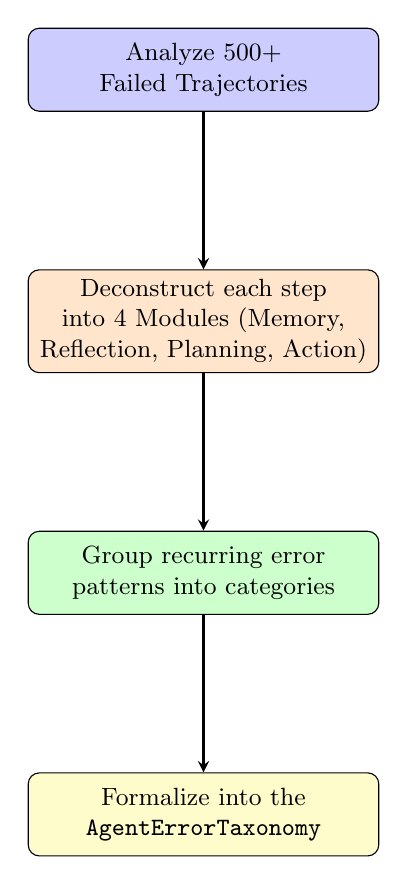
\begin{tikzpicture}[node distance=2cm, font=\small]
    \node (p1) [wideblock, fill=blue!20] {Analyze 500+ Failed Trajectories};
    \node (p2) [wideblock, fill=orange!20, below=of p1] {Deconstruct each step into 4 Modules (Memory, Reflection, Planning, Action)};
    \node (p3) [wideblock, fill=green!20, below=of p2] {Group recurring error patterns into categories};
    \node (p4) [wideblock, fill=yellow!20, below=of p3] {Formalize into the \texttt{AgentErrorTaxonomy}};

    \draw [arrow] (p1) -- (p2);
    \draw [arrow] (p2) -- (p3);
    \draw [arrow] (p3) -- (p4);
  \end{tikzpicture}
  \end{center}
\end{frame}

\begin{frame}[fragile]
  \frametitle{The Full \texttt{AgentErrorTaxonomy} (1/3): Memory}
  \textbf{Memory:} Errors in recalling or retrieving information.
  \begin{description}
    \item[Over-simplification / Incomplete Summary] Summarizes past info too crudely, ignoring critical details.
    \begin{itemize}
        \item \textit{Example:} Agent is told "find a red shirt, size medium." Its memory becomes "find a shirt," forgetting the constraints.
    \end{itemize}
    \vfill
    \item[Hallucination (False Memory)] Recalls events or states that never happened.
    \begin{itemize}
        \item \textit{Example:} After a failed API call, the agent "remembers" that the call was successful and returned data.
    \end{itemize}
    \vfill
    \item[Retrieval Failure] Relevant information exists in the agent's history, but it fails to retrieve it when needed.
    \begin{itemize}
        \item \textit{Example:} The user provided an API key on step 1, but on step 5 the agent asks for the key again.
    \end{itemize}
  \end{description}
\end{frame}

\begin{frame}[fragile]
  \frametitle{The Full \texttt{AgentErrorTaxonomy} (2/3): Reflection \& Planning}
  \textbf{Reflection:} Errors in monitoring progress or interpreting outcomes.
  \begin{description}
    \item[Progress Misassessment] Incorrectly evaluates its own progress (e.g., thinks it's done when it's not).
    \item[Outcome Misinterpretation] Correctly executes an action but misreads the feedback from the environment.
    \item[Causal Misattribution] Correctly notes a failure but blames the wrong cause.
  \end{description}
  
  \vfill
  
  \textbf{Planning:} Errors in formulating a strategy.
  \begin{description}
    \item[Constraint Ignorance] Ignores limits (time, budget, user rules) when forming a plan.
    \item[Impossible Action] Plans a step that is physically or logically impossible.
    \item[Inefficient Planning] The plan is overly long, illogical, or wastes steps.
  \end{description}
\end{frame}

\begin{frame}[fragile]
  \frametitle{The Full \texttt{AgentErrorTaxonomy} (3/3): Action \& System}
  \textbf{Action:} Errors in executing an operation.
  \begin{description}
    \item[Planning-Action Disconnect] The chosen action does not align with the agent's stated plan.
    \item[Format Error] Produces a syntactically invalid action (e.g., malformed JSON).
    \item[Parameter Error] Generates an action with unreasonable or malformed parameters.
  \end{description}
  
  \vfill
  
  \textbf{System-level:} Failures caused by the external environment or tools.
  \begin{description}
    \item[Step Limit Exhaustion] Fails by reaching the maximum step count.
    \item[Tool Execution Error] An external tool/API crashes or returns an error.
    \item[Environment Error] The environment itself breaks or does not follow expected rules.
  \end{description}
\end{frame}

% --- PART 3: THE FRAMEWORK ---
\part{The AgentDebug Framework}

\begin{frame}
  \frametitle{The \texttt{AgentDebug} Framework: A Step-by-Step Guide}
  With a taxonomy in place, we can build a system to automatically find and fix errors.
  
  \begin{center}
  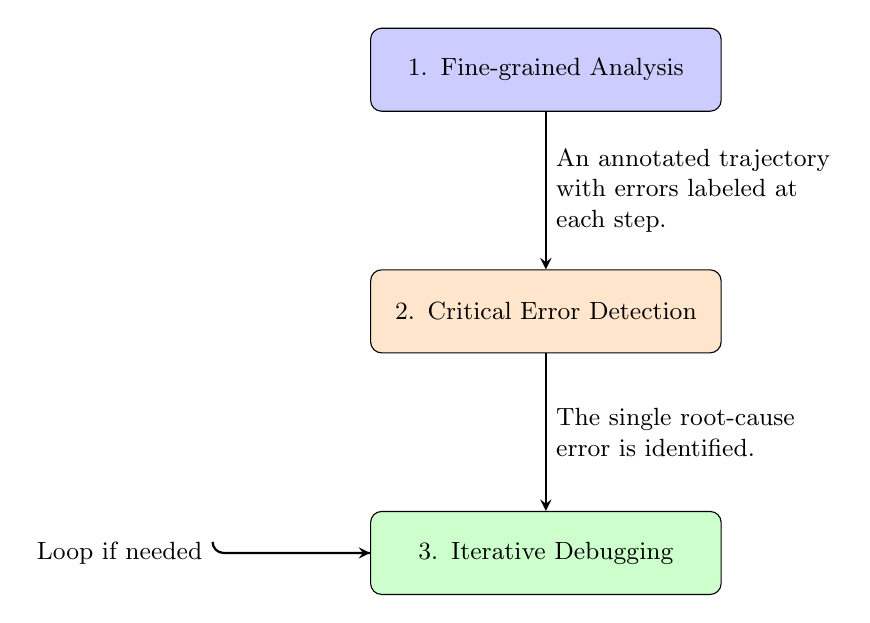
\begin{tikzpicture}[node distance=2cm, font=\small]
    \node (p1) [wideblock, fill=blue!20] {1. Fine-grained Analysis};
    \node (p2) [wideblock, fill=orange!20, below=of p1] {2. Critical Error Detection};
    \node (p3) [wideblock, fill=green!20, below=of p2] {3. Iterative Debugging};

    \draw [arrow] (p1) -- node[right, text width=10em] {An annotated trajectory with errors labeled at each step.} (p2);
    \draw [arrow] (p2) -- node[right, text width=10em] {The single root-cause error is identified.} (p3);
    \draw [arrow, rounded corners] (p3.west) -- ++(-2,0) |- node[left] {Loop if needed} (p3.west);
  \end{tikzpicture}
  \end{center}
\end{frame}

\begin{frame}
  \frametitle{Framework Deep Dive: Critical Error Detection}
  This is the core of \texttt{AgentDebug}. It's not about finding all errors, but about finding the \textbf{one} that mattered most.
  
  \textbf{The "Counterfactual" Question:}
  The system asks for each step `t` in the trajectory: \textit{"If the agent had done the right thing at step `t`, would the rest of the trajectory have succeeded?"}
  
  \begin{center}
  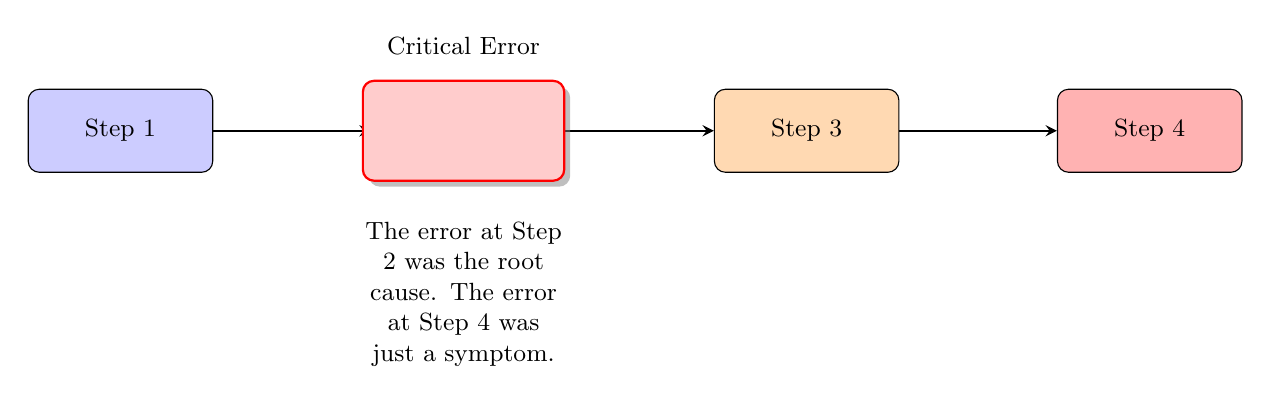
\begin{tikzpicture}[font=\small]
    \node (t1) [block, fill=blue!20] {Step 1};
    \node (t2) [block, fill=red!30, right=of t1, xshift=1cm] {Step 2};
    \node (t3) [block, fill=orange!30, right=of t2, xshift=1cm] {Step 3};
    \node (t4) [block, fill=red!30, right=of t3, xshift=1cm] {Step 4};
    
    \draw[arrow] (t1) -- (t2);
    \draw[arrow] (t2) -- (t3);
    \draw[arrow] (t3) -- (t4);
    
    \node[highlight, fit=(t2), inner sep=0.1cm, label={[yshift=0.2cm]above:Critical Error}] {};
    \node[note, below=0.5cm of t2] {The error at Step 2 was the root cause. The error at Step 4 was just a symptom.};
  \end{tikzpicture}
  \end{center}
  
  The \textbf{Critical Error} is the \textit{earliest} step where the answer is "Yes." This prevents wasting time fixing downstream symptoms of an earlier, deeper mistake.
\end{frame}

\begin{frame}
  \frametitle{Framework Deep Dive: Iterative Debugging}
  Once the root cause is found, \texttt{AgentDebug} generates targeted feedback and re-runs the agent from that critical point.
  
  \begin{center}
  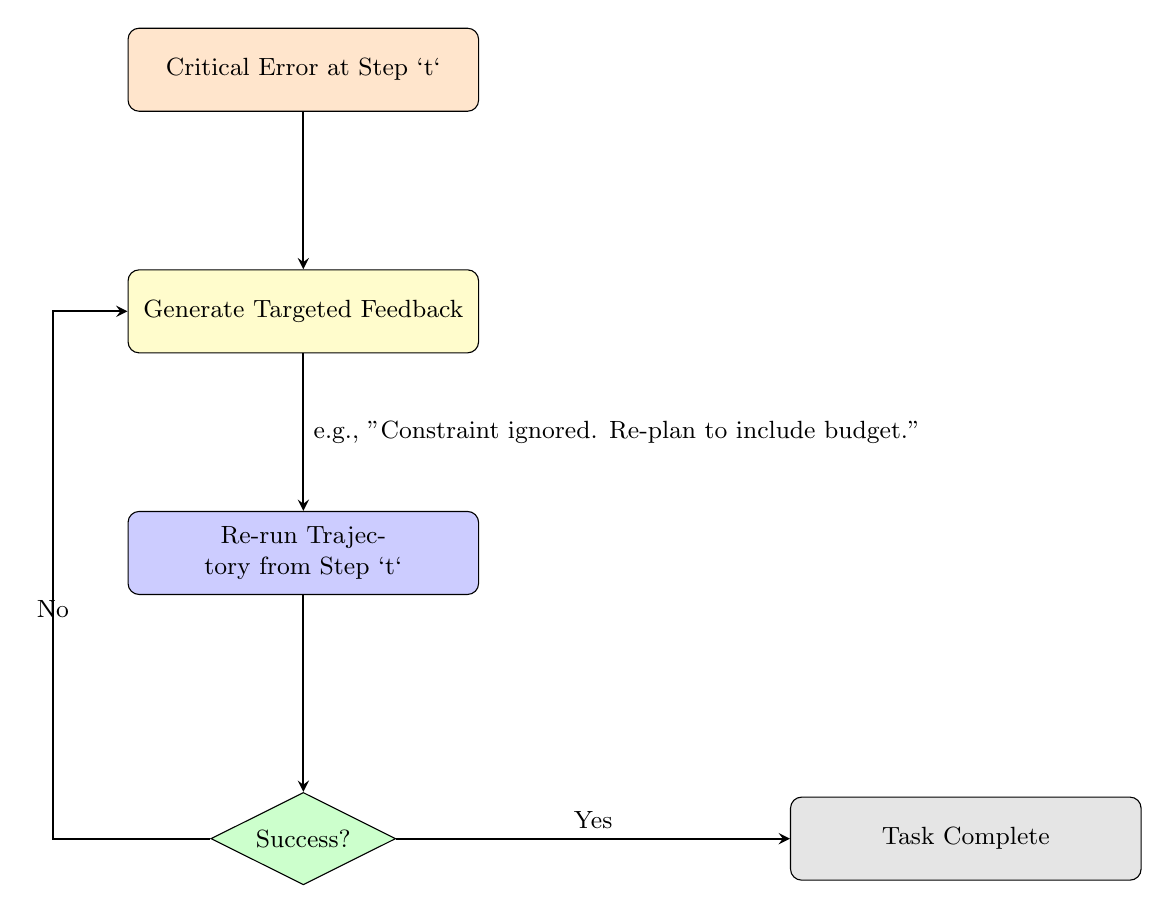
\begin{tikzpicture}[node distance=2cm, font=\small]
    \node (start) [wideblock, fill=orange!20] {Critical Error at Step `t`};
    \node (feedback) [wideblock, fill=yellow!20, below=of start] {Generate Targeted Feedback};
    \node (rerun) [wideblock, fill=blue!20, below=of feedback] {Re-run Trajectory from Step `t`};
    \node (eval) [diamond, aspect=2, draw, fill=green!20, below=of rerun, yshift=-0.5cm] {Success?};
    \node (end) [wideblock, fill=gray!20, right=of eval, xshift=3cm] {Task Complete};
    
    \draw[arrow] (start) -- (feedback);
    \draw[arrow] (feedback) -- node[right] {e.g., "Constraint ignored. Re-plan to include budget."} (rerun);
    \draw[arrow] (rerun) -- (eval);
    \draw[arrow] (eval) -- node[above] {Yes} (end);
    \draw[arrow] (eval.west) -- ++(-2,0) |- node[above, pos=0.2] {No} (feedback.west);
  \end{tikzpicture}
  \end{center}
\end{frame}

\begin{frame}
  \frametitle{Experimental Validation: Does It Work?}
  Yes. The paper shows that this principled debugging approach significantly improves task success compared to baselines.
  
  \begin{center}
    \textbf{Key Finding from Paper's Experiments}
    \vfill
    \textit{--- Insert Figure 5 from AgentDebug (Zhu et al., 2025) here. ---} \\
    \includegraphics[width=\textwidth]{placeholder.png} \\
    \small{Performance of \texttt{AgentDebug} vs. other methods on the ALFWorld benchmark.}
  \end{center}
  
  \textbf{The Takeaway:} Precisely identifying and correcting the root-cause failure is far more effective than unguided self-reflection or simply trying more times.
\end{frame}

% --- PART 4: MAST EXAMPLES ---
\part{Multi-Agent Failure Cases}

\begin{frame}
  \frametitle{A Glimpse into Multi-Agent Failures}
  While \texttt{AgentDebug} focuses on single agents, the \texttt{MAST} paper (Cemri et al., 2025) provides great examples of failures unique to \textbf{multi-agent systems}.
  
  \vfill
  
  In MAS, failures often stem from flawed \textbf{communication} and \textbf{coordination}, not just individual reasoning.
\end{frame}

\begin{frame}
  \frametitle{MAS Failure Case: Information Withholding}
  \textbf{Category:} Inter-Agent Misalignment (Agents fail to coordinate effectively).
  
  \begin{center}
  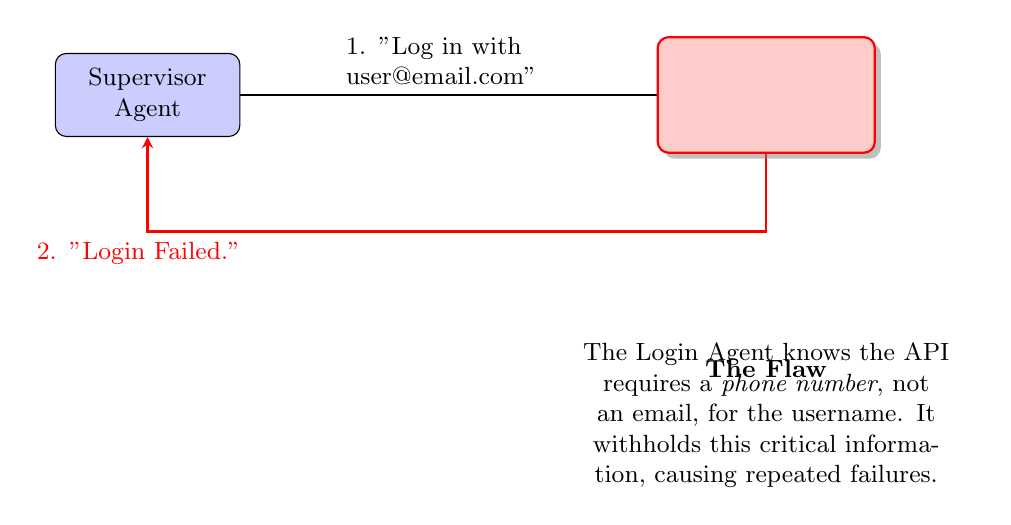
\begin{tikzpicture}[node distance=1.5cm, font=\small]
    \node (sup) [block, fill=blue!20] {Supervisor Agent};
    \node (login) [block, fill=orange!20, right=of sup, xshift=4cm] {Login Agent};
    
    \draw[arrow] (sup) -- node[midway, above, text width=8em] {1. "Log in with user@email.com"} (login);
    \draw[arrow, color=red] (login.south) -- ++(0,-1.2) -| (sup.south) node[midway, below, text width=8em] {2. "Login Failed."};
    
    \node[highlight, fill=red!20, draw=red, fit=(login), inner sep=0.2cm, label={[yshift=-2.5cm]below:\textbf{The Flaw}}] {};
    \node[note, text width=15em, below=2.5cm of login] {The Login Agent knows the API requires a \textit{phone number}, not an email, for the username. It withholds this critical information, causing repeated failures.};
  \end{tikzpicture}
  \end{center}
  This is a communication failure. The system as a whole fails because the agents do not share necessary context to help each other succeed.
\end{frame}

\begin{frame}
  \frametitle{MAS Failure Case: Incorrect Verification}
  \textbf{Category:} Task Verification (The system fails to properly check its own work).
  
  \begin{center}
  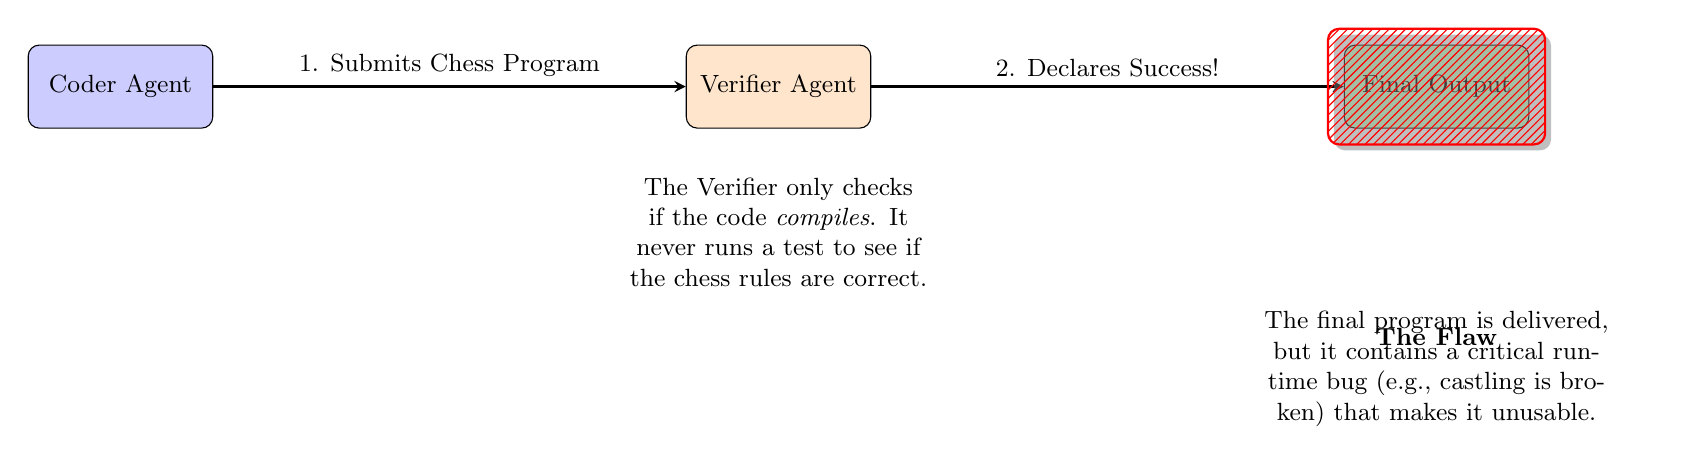
\begin{tikzpicture}[node distance=2cm, font=\small]
    \node (coder) [block, fill=blue!20] {Coder Agent};
    \node (verifier) [block, fill=orange!20, right=of coder, xshift=4cm] {Verifier Agent};
    \node (output) [block, fill=green!20, right=of verifier, xshift=4cm] {Final Output};
    
    \draw[arrow] (coder) -- node[midway, above] {1. Submits Chess Program} (verifier);
    \draw[arrow] (verifier) -- node[midway, above] {2. Declares Success!} (output);
    
    \node[note, text width=12em, below=0.5cm of verifier] (note_verifier) {The Verifier only checks if the code \textit{compiles}. It never runs a test to see if the chess rules are correct.};
    
    \node[highlight, pattern=north east lines, pattern color=red, fit=(output), inner sep=0.2cm, label={[yshift=-2.2cm]below:\textbf{The Flaw}}] {};
    \node[note, text width=15em, below=2.2cm of output] {The final program is delivered, but it contains a critical runtime bug (e.g., castling is broken) that makes it unusable.};
  \end{tikzpicture}
  \end{center}
  The system prematurely declares success because its verification process was too superficial.
\end{frame}

% --- PART 5: CONCLUSION ---
\part{Conclusion}

\begin{frame}
  \frametitle{Conclusion \& Key Takeaways}
  
  \begin{enumerate}
    \item \textbf{Failure is Systemic, Not Just Local} \\ Errors are rarely isolated. They propagate within a single agent's reasoning and emerge from flawed interactions between multiple agents.
    \vfill
    \item \textbf{A Taxonomy is a Prerequisite for Debugging} \\ We need a precise language to describe failures before we can build tools to fix them. The \texttt{AgentErrorTaxonomy} provides this for single agents.
    \vfill
    \item \textbf{Root Cause Analysis is Essential} \\ Fixing surface-level symptoms is not enough. Effective debugging, as demonstrated in \texttt{AgentDebug}, must find and correct the single, earliest point of failure.
    \vfill
    \item \textbf{Automation is the Goal} \\ Frameworks like \texttt{AgentDebug} are the first step towards creating agents that can learn from their own mistakes and become truly robust and reliable.
  \end{enumerate}
\end{frame}

% --- REFERENCES ---
\begin{frame}[allowframebreaks]
  \frametitle{References}
  \begin{thebibliography}{99}
    \bibitem{agentdebug}
    Zhu, K., Liu, Z., Li, B., et al. (2025).
    \newblock \textit{WHERE LLM AGENTS FAIL AND HOW THEY CAN LEARN FROM FAILURES}.
    \newblock arXiv:2509.25370v1.
    
    \bibitem{mast}
    Cemri, M., Pan, M. Z., Yang, S., et al. (2025).
    \newblock \textit{Why Do Multi-Agent LLM Systems Fail?}.
    \newblock arXiv:2503.13657v3.
    
  \end{thebibliography}
\end{frame}

% --- Q&A SLIDE ---
\begin{frame}
  \frametitle{Thank You}
  \begin{center}
    \huge \textbf{Questions?}
  \end{center}
\end{frame}

\end{document}